% !TEX program = pdflatex
% -----------------------------------------------------------------------------
% Laboratorio 3 - Gramaticas Libres de Contexto (INFO1148)
% Version LaTeX adaptada al formato de informe entregado por el docente.
% Compilar con pdfLaTeX.
%
% La imagen arbol_z_igual_x_mas_y.png debe estar en la misma carpeta que este
% archivo (o en ../gramatica/salidas/). En Overleaf: subir el .tex y el .png.
% -----------------------------------------------------------------------------
\documentclass[11pt,letterpaper]{article}

\usepackage[utf8]{inputenc}
\usepackage[T1]{fontenc}
% En Overleaf se puede agregar, para mejorar la particion de palabras:
% \usepackage[spanish,es-noshorthands]{babel}
\usepackage{mathptmx}
\usepackage[scaled=0.92]{helvet}
\usepackage[letterpaper,margin=2.54cm]{geometry}
\usepackage{amsmath,amssymb}
\usepackage{graphicx}
\usepackage{array}
\usepackage{longtable}
\usepackage{tabularx}
\usepackage{xcolor}
\usepackage{colortbl}
\usepackage{ragged2e}
\usepackage{enumitem}
\usepackage{fancyhdr}
\usepackage{titlesec}
\usepackage{caption}
\usepackage{listings}
\usepackage{float}
\usepackage{hyperref}
\usepackage{newunicodechar}
\usepackage{microtype}
\usepackage{textcomp}
\usepackage{needspace}

% --- Caracteres Unicode usados en el informe -------------------------------
\newunicodechar{ε}{\ensuremath{\varepsilon}}
\newunicodechar{Σ}{\ensuremath{\Sigma}}
\newunicodechar{⇒}{\ensuremath{\Rightarrow}}
\newunicodechar{∈}{\ensuremath{\in}}
\newunicodechar{≤}{\ensuremath{\leq}}
\newunicodechar{≥}{\ensuremath{\geq}}
\newunicodechar{≠}{\ensuremath{\neq}}
\newunicodechar{✔}{\ensuremath{\checkmark}}

% --- Paleta del formato -----------------------------------------------------
\definecolor{azul}{RGB}{46,116,181}
\definecolor{azuloscuro}{RGB}{31,78,121}
\definecolor{azulclaro}{RGB}{222,234,246}
\definecolor{grisfondo}{RGB}{247,249,251}
\definecolor{grisborde}{RGB}{190,200,210}

\hypersetup{
  colorlinks=true,
  linkcolor=azul,
  urlcolor=azul,
  citecolor=azul,
  pdftitle={Informe de Laboratorio 3 - Gramaticas Libres de Contexto},
  pdfauthor={Francisco Benavides, Marcelo Matamala}
}

\lstset{
  basicstyle=\ttfamily\footnotesize,
  breaklines=true,
  breakatwhitespace=false,
  breakindent=1em,
  columns=fullflexible,
  keepspaces=true,
  showstringspaces=false,
  frame=single,
  rulecolor=\color{grisborde},
  backgroundcolor=\color{grisfondo},
  xleftmargin=0.3em,
  xrightmargin=0.3em,
  aboveskip=0.5em,
  belowskip=0.5em,
  literate={ε}{{$\varepsilon$}}1
           {Σ}{{$\Sigma$}}1
           {⇒}{{$\Rightarrow$}}1
           {→}{{$\rightarrow$}}1
           {∈}{{$\in$}}1
           {…}{{\ldots}}1
           {≤}{{$\leq$}}1
           {≥}{{$\geq$}}1
           {≠}{{$\neq$}}1
}

\newcolumntype{L}[1]{>{\RaggedRight\arraybackslash}p{#1}}
\newcolumntype{C}[1]{>{\centering\arraybackslash}p{#1}}

% Etiqueta de subsección a), b), c) del formato del docente.
\newcommand{\letra}[2]{\par\medskip\noindent #1)~#2\par\smallskip}

% Tablas con el mismo borde y tamano reducido del formato.
\newenvironment{tabla}[1]{\par\small\begin{longtable}{#1}}{\end{longtable}\par}
\newenvironment{tablaf}[1]{\par\footnotesize\begin{longtable}{#1}}{\end{longtable}\par}

% --- Títulos azules, sans-serif, como el formato de referencia --------------
\titleformat{\section}{\sffamily\Large\bfseries\color{azul}}{\thesection.}{0.5em}{}
\titleformat{\subsection}{\sffamily\large\bfseries\color{azul}}{\thesubsection}{0.5em}{}
\titlespacing*{\section}{0pt}{1.4em}{0.7em}
\titlespacing*{\subsection}{0pt}{1.1em}{0.4em}

\captionsetup{font=small,labelfont=bf,labelsep=period}
\renewcommand{\figurename}{Figura}
\renewcommand{\tablename}{Tabla}
\setlength{\parindent}{0pt}
\setlength{\parskip}{0.5em}
\renewcommand{\arraystretch}{1.15}
\setlength{\arrayrulewidth}{0.5pt}
\setlength{\tabcolsep}{4pt}
\emergencystretch=2em

% --- Pie de página con el número, sin encabezado ---------------------------
\pagestyle{fancy}
\fancyhf{}
\renewcommand{\headrulewidth}{0pt}
\fancyfoot[R]{\thepage}

\graphicspath{{./}{../gramatica/salidas/}{gramatica/salidas/}{salidas/}}

\begin{document}

% =============================== PORTADA ====================================
\begin{center}
  {\Large\bfseries INFORME DE LABORATORIO \# 3}\\[0.35em]
  {\large\bfseries Gramáticas Libres de Contexto}
\end{center}

\vspace{0.5em}

\begin{center}
\begin{tabularx}{0.95\textwidth}{|p{0.27\textwidth}|X|}
\hline
\rowcolor{azuloscuro}
\multicolumn{1}{|c|}{\textcolor{white}{\textbf{Antecedente}}} &
\multicolumn{1}{c|}{\textcolor{white}{\textbf{Información}}}\\
\hline
Asignatura & Teoría de la Computación -- INFO1148\\
\hline
Carrera & Ingeniería Civil en Informática\\
\hline
Docente & Marcos Lévano\\
\hline
Integrantes & Francisco Benavides; Marcelo Matamala\\
\hline
Fecha & 24 de octubre de 2026\\
\hline
\end{tabularx}
\end{center}

% =============================== 1. INTRODUCCION ===========================
\section{Introducción}

El objetivo de este laboratorio es diseñar, analizar y validar una gramática libre de contexto (GLC) que
represente la estructura sintáctica de un lenguaje de programación simplificado. Se identifican sus
componentes formales (terminales, no terminales y símbolo inicial), se construyen las producciones, se
realizan derivaciones por la izquierda, se construye el árbol sintáctico y se comprueba la pertenencia de
cadenas válidas e inválidas.

El lenguaje de referencia incluye un bloque \lstinline|Begin ... End|, un identificador de programa,
asignaciones simples y aritméticas, instrucciones de salida, comentarios y una o más instrucciones por
programa. La gramática se implementó en \lstinline|gramatica.py| y la evidencia de ejecución se conserva en
\lstinline|validacion.txt|. Como extensión creativa se agrega el condicional
\lstinline|si ... entonces ... fin_si|.

% =============================== 2. DESARROLLO =============================
\section{Desarrollo}

\subsection{Pregunta 1 -- Componentes de la gramática}

\letra{a}{Símbolos terminales}

El alfabeto de la gramática es \textbf{finito} y está formado por lexemas fijos y por clases de token que
representan conjuntos infinitos de lexemas:

\begin{tabla}{|L{0.24\textwidth}|L{0.68\textwidth}|}
\hline
\rowcolor{azulclaro}
\textbf{Categoría} & \textbf{Elementos identificados}\\
\hline
\endhead
Palabras reservadas & \lstinline|Begin|, \lstinline|End|, \lstinline|Programa|, \lstinline|salida|,
\lstinline|si|, \lstinline|entonces|, \lstinline|fin_si|\\
\hline
Operadores & \lstinline|+|, \lstinline|-|, \lstinline|*|, \lstinline|/|, \lstinline|%|;
\lstinline|<|, \lstinline|>|, \lstinline|<=|, \lstinline|>=|, \lstinline|==|, \lstinline|!=|;
\lstinline|=|\\
\hline
Símbolos especiales & \lstinline|#| (terminador obligatorio de instrucción)\\
\hline
Identificadores & \lstinline|ID|: \lstinline|[a-zA-Z][a-zA-Z0-9_]*|; comienza con letra y admite letras,
dígitos y guion bajo\\
\hline
Números & \lstinline|NUM|: \lstinline|[0-9]+("."[0-9]+)?|; enteros o reales positivos, sin signo\\
\hline
Comentarios & \lstinline|COMENT|: \lstinline|/* ... */|, tratado como un solo token\\
\hline
\end{tabla}

\textbf{Convención léxica.} Los espacios, tabuladores y saltos de línea no pertenecen al lenguaje: el
analizador léxico los descarta antes de aplicar las producciones. El espacio en blanco no se incluye en
$\Sigma$ porque no aporta estructura sintáctica.

\letra{b}{Símbolos no terminales}

El conjunto de no terminales es:

\begin{center}
$V = \{$ \lstinline|<programa>|, \lstinline|<lista_instrucciones>|, \lstinline|<resto_lista>|,
\lstinline|<instruccion>|, \lstinline|<asignacion>|, \lstinline|<asignacion_simple>|,
\lstinline|<asignacion_aritmetica>|, \lstinline|<expresion_aritmetica>|,
\lstinline|<resto_expresion_aritmetica>|, \lstinline|<termino_aritmetico>|,
\lstinline|<resto_termino_aritmetico>|, \lstinline|<expresion>|, \lstinline|<resto_expresion>|,
\lstinline|<termino>|, \lstinline|<resto_termino>|, \lstinline|<factor>|, \lstinline|<operando>|,
\lstinline|<salida>|, \lstinline|<identificador>|, \lstinline|<numero>|, \lstinline|<comentario>|,
\lstinline|<condicional>|, \lstinline|<condicion>|, \lstinline|<operador_relacional>| $\}$
\quad $\Rightarrow$ \quad $|V| = 24$.
\end{center}

\letra{c}{Símbolo inicial}

$S =$ \lstinline|<programa>|. Es el único no terminal que produce un programa completo (desde
\lstinline|Begin| hasta \lstinline|End|), por lo que toda cadena del lenguaje debe derivarse a partir de él.

\letra{d}{Definición formal de la gramática}

$G = (V, \Sigma, P, S)$, donde:

$V = \{$ conjunto de 24 no terminales de la sección 2.1 b) $\}$.

$\Sigma = \{$ \lstinline|Begin|, \lstinline|End|, \lstinline|Programa|, \lstinline|salida|,
\lstinline|si|, \lstinline|entonces|, \lstinline|fin_si|, \lstinline|+ - * / %|,
\lstinline|< > <= >= == !=|, \lstinline|=|, \lstinline|#|, \lstinline|ID|, \lstinline|NUM|,
\lstinline|COMENT| $\}$.

$P =$ conjunto de las \textbf{45 producciones} desarrolladas en la sección 2.2 a): \textbf{36 del núcleo}
(P1--P8 y P10--P37) y \textbf{9 de la extensión} (P9 y P38--P45).

$S =$ \lstinline|<programa>|.

\letra{e}{Análisis}

Los identificadores y los números son conjuntos \textbf{infinitos}, mientras que una gramática es un objeto
\textbf{finito}. Por eso se modelan como clases de token (\lstinline|ID|, \lstinline|NUM| y
\lstinline|COMENT|) reconocidas por reglas regulares. Así, $\Sigma$ y $P$ permanecen finitos y la gramática
describe un lenguaje, no una lista cerrada de programas.

Enumerar cada identificador o cada número haría que $P$ fuera infinita: habría que escribir una producción
para \lstinline|x|, otra para \lstinline|y|, otra para \lstinline|temporal|, y así para cada nombre y cada
valor posible. Además, un programa que use un identificador nuevo (\lstinline|contador_02|) quedaría fuera del
lenguaje aunque sea sintácticamente idéntico a uno ya enumerado. La separación entre análisis léxico y
análisis sintáctico evita ese problema: el lexer decide si una cadena es \lstinline|ID| o \lstinline|NUM| y
la GLC trabaja sobre tokens. Gracias a esa abstracción, \lstinline|x = 20 #| y
\lstinline|operativo_01_02 = 1.345 #| se derivan con las mismas producciones (P10, P12, P32/P33, P35/P36);
solo cambia el lexema asociado al token.

Los comentarios se tratan de la misma manera: \lstinline|COMENT| es un único terminal, aunque su contenido
pueda incluir cualquier carácter. Modelarlos carácter por carácter exigiría producciones para todo el
alfabeto y no aportaría estructura sintáctica. Se admiten comentarios antes, entre y después de las
instrucciones, pero no un programa formado solo por comentarios: la producción P2 no tiene alternativa
$\varepsilon$, de modo que tras un comentario inicial siempre se exige una lista que desemboque en una
instrucción (P3).

\subsection{Pregunta 2 -- Construcción de la Gramática Libre de Contexto}

\letra{a}{Producciones propuestas}

La gramática tiene 45 producciones: 36 del núcleo (P1--P8 y P10--P37) y 9 de la extensión (P9 y P38--P45).
En la tabla se agrupan por no terminal; cada línea de la columna derecha es una producción distinta.

\begin{tablaf}{|L{0.32\textwidth}|L{0.60\textwidth}|}
\hline
\rowcolor{azulclaro}
\textbf{No terminal} & \textbf{Producción}\\
\hline
\endhead
\lstinline|<programa>| & \lstinline|Begin Programa <identificador>| \newline
\lstinline|<lista_instrucciones> End|\\
\hline
\lstinline|<lista_instrucciones>| & \lstinline|<comentario> <lista_instrucciones>| \newline
\lstinline|<instruccion> <resto_lista>|\\
\hline
\lstinline|<resto_lista>| & \lstinline|<instruccion> <resto_lista>| \newline
\lstinline|<comentario> <resto_lista>| \newline \(\varepsilon\)\\
\hline
\lstinline|<instruccion>| & \lstinline|<asignacion>| \newline \lstinline|<salida>| \newline
\lstinline|<condicional>| \textbf{(ext.)}\\
\hline
\lstinline|<asignacion>| & \lstinline|<asignacion_simple>| \newline \lstinline|<asignacion_aritmetica>|\\
\hline
\lstinline|<asignacion_simple>| & \lstinline|<identificador> = <operando> #|\\
\hline
\lstinline|<asignacion_aritmetica>| & \lstinline|<identificador> = <expresion_aritmetica> #|\\
\hline
\lstinline|<expresion_aritmetica>| & \lstinline|<termino> <resto_expresion_aritmetica>| \newline
\lstinline|<termino_aritmetico>|\\
\hline
\lstinline|<resto_expresion_aritmetica>| & \lstinline|+ <termino> <resto_expresion>| \newline
\lstinline|- <termino> <resto_expresion>|\\
\hline
\lstinline|<termino_aritmetico>| & \lstinline|<factor> <resto_termino_aritmetico>|\\
\hline
\lstinline|<resto_termino_aritmetico>| & \lstinline|* <factor> <resto_termino>| \newline
\lstinline|/ <factor> <resto_termino>| \newline
\lstinline|% <factor> <resto_termino>|\\
\hline
\lstinline|<expresion>| & \lstinline|<termino> <resto_expresion>|\\
\hline
\lstinline|<resto_expresion>| & \lstinline|+ <termino> <resto_expresion>| \newline
\lstinline|- <termino> <resto_expresion>| \newline \(\varepsilon\)\\
\hline
\lstinline|<termino>| & \lstinline|<factor> <resto_termino>|\\
\hline
\lstinline|<resto_termino>| & \lstinline|* <factor> <resto_termino>| \newline
\lstinline|/ <factor> <resto_termino>| \newline
\lstinline|% <factor> <resto_termino>| \newline \(\varepsilon\)\\
\hline
\lstinline|<factor>| & \lstinline|<operando>|\\
\hline
\lstinline|<operando>| & \lstinline|<identificador>| \newline \lstinline|<numero>|\\
\hline
\lstinline|<salida>| & \lstinline|salida <identificador> #|\\
\hline
\lstinline|<identificador>| & \lstinline|ID|\\
\hline
\lstinline|<numero>| & \lstinline|NUM|\\
\hline
\lstinline|<comentario>| & \lstinline|COMENT|\\
\hline
\lstinline|<condicional>| \textbf{(ext.)} & \lstinline|si <condicion> entonces| \newline
\lstinline|<lista_instrucciones> fin_si|\\
\hline
\lstinline|<condicion>| \textbf{(ext.)} & \lstinline|<expresion> <operador_relacional> <expresion>|\\
\hline
\lstinline|<operador_relacional>| \textbf{(ext.)} & \lstinline|<| \newline \lstinline|>| \newline
\lstinline|<=| \newline \lstinline|>=| \newline \lstinline|==| \newline \lstinline|!=|\\
\hline
\end{tablaf}

\needspace{4\baselineskip}
La misma gramática, en formato BNF listo para copiar en otra herramienta, está en:

\begin{center}
\path{gramatica/Lab3_gramatica.bnf}
\end{center}

La numeración completa P1--P45 se conserva en ese archivo y en la evidencia de ejecución.

\letra{b}{Explicación de los no terminales}

\begin{tabla}{|L{0.30\textwidth}|L{0.62\textwidth}|}
\hline
\rowcolor{azulclaro}
\textbf{No terminal} & \textbf{Función dentro de la gramática}\\
\hline
\endhead
\lstinline|<programa>| & Unidad sintáctica completa: \lstinline|Begin Programa <id> <instrucciones> End|.\\
\hline
\lstinline|<lista_instrucciones>| & Inicia la lista con al menos una instrucción (P3), admitiendo comentarios
previos (P2).\\
\hline
\lstinline|<resto_lista>| & Continúa la lista con más instrucciones (P4), más comentarios (P5) o la cierra con
$\varepsilon$ (P6).\\
\hline
\lstinline|<instruccion>| & Uniformiza el contenido de la lista y concentra la decisión entre asignación,
salida y condicional (P7--P9).\\
\hline
\lstinline|<asignacion>| & Separa la decisión simple/aritmética del resto (P10/P11).\\
\hline
\lstinline|<asignacion_simple>| & Reconoce asignaciones de un solo valor (P12).\\
\hline
\lstinline|<asignacion_aritmetica>| & Reconoce asignaciones con al menos una operación (P13).\\
\hline
\lstinline|<expresion_aritmetica>| & Obliga a que exista al menos un operador; sin ella no se podría
distinguir la asignación simple.\\
\hline
\lstinline|<resto_expresion_aritmetica>| & Aporta el primer \lstinline|+|/\lstinline|-| de nivel superior y
encadena el resto con \lstinline|<resto_expresion>| (P16/P17).\\
\hline
\lstinline|<termino_aritmetico>| & Aporta al menos un \lstinline|*|, \lstinline|/| o \lstinline|%| cuando no
hay sumas/restas (P18).\\
\hline
\lstinline|<resto_termino_aritmetico>| & Encadena los operadores multiplicativos y exige al menos uno
(P19--P21).\\
\hline
\lstinline|<expresion>| & Nivel aditivo del núcleo: agrupa términos con \lstinline|+|/\lstinline|-|
(P22--P25).\\
\hline
\lstinline|<resto_expresion>| & Recursión del nivel aditivo y caso base $\varepsilon$ (P23--P25).\\
\hline
\lstinline|<termino>| & Nivel multiplicativo del núcleo: agrupa factores con \lstinline|*|, \lstinline|/|,
\lstinline|%| (P26--P30).\\
\hline
\lstinline|<resto_termino>| & Recursión del nivel multiplicativo y caso base $\varepsilon$ (P27--P30).\\
\hline
\lstinline|<factor>| & Unidad de la expresión; permite ampliar el lenguaje (por ejemplo, paréntesis) sin
tocar los demás niveles (P31).\\
\hline
\lstinline|<operando>| & Único punto donde se elige entre identificador y número (P32/P33).\\
\hline
\lstinline|<salida>| & Estructura propia de impresión (P34).\\
\hline
\lstinline|<identificador>| & Enlace con el token \lstinline|ID|; mantiene la gramática independiente de los
lexemas concretos (P35).\\
\hline
\lstinline|<numero>| & Enlace con el token \lstinline|NUM| (enteros y reales) (P36).\\
\hline
\lstinline|<comentario>| & Enlace con el token \lstinline|COMENT|; permite comentarios sin contaminar las
instrucciones (P37).\\
\hline
\lstinline|<condicional>| & (Ext.) Estructura de control con condición y bloque propio (P38).\\
\hline
\lstinline|<condicion>| & (Ext.) Separa la condición del bloque para que sea reutilizable (P39).\\
\hline
\lstinline|<operador_relacional>| & (Ext.) Agrupa las seis comparaciones (P40--P45).\\
\hline
\end{tabla}

\letra{c}{Verificación de la gramática}

El programa de referencia es el siguiente:

\begin{lstlisting}
Begin
Programa operativo_01_02

x = 1.345 #
y = 20 #

/* operaciones y salidas */

z = x + y #
z2 = x + y #
h = z - x #
h2 = z - x #
k = h * y #
t = k / z #
m = k % 10 #

salida z #
salida h #
salida k #
salida t #
salida m #

temporal = 0 #
temporal = x #
x = y #
y = temporal #

salida x #
salida y #

End
\end{lstlisting}

\textbf{Sí, la gramática representa el programa de referencia completo.} El validador lo procesa y responde
\textbf{ACEPTADO}, contando los elementos reconocidos:

\begin{tabla}{|L{0.42\textwidth}|L{0.34\textwidth}|C{0.16\textwidth}|}
\hline
\rowcolor{azulclaro}
\textbf{Elemento del programa} & \textbf{Producciones aplicadas} & \textbf{Cantidad}\\
\hline
\endhead
\lstinline|Begin| ... \lstinline|End| con identificador & P1 + P35 & 1 programa\\
\hline
Asignaciones simples & P10, P12, P32/P33, P35/P36 & \textbf{6}\\
\hline
Asignaciones aritméticas & P11, P13, P14/P15 & \textbf{7}\\
\hline
Salidas & P34 + P35 & \textbf{7}\\
\hline
Comentario \lstinline|/* operaciones y salidas */| & P5 + P37 & \textbf{1}\\
\hline
\textbf{Total de elementos de la lista} & P2--P6 & \textbf{21}\\
\hline
\end{tabla}

Los números coinciden con el programa: 20 instrucciones + 1 comentario = 21 elementos. Además, los números
\lstinline|1.345| (real) y \lstinline|20|, \lstinline|0|, \lstinline|10| (enteros) se aceptan con la misma
clase \lstinline|NUM| (P36), lo que confirma que no hace falta enumerar valores. El árbol completo exportado
en \lstinline|arbol_programa_referencia.dot| incluye los nodos \lstinline|<resto_lista>| de P3--P6.

\subsection{Pregunta 3 -- Derivaciones y árbol sintáctico}

\letra{a}{Derivación por la izquierda para: \texttt{z=x+y\#}}

Convención: $\Rightarrow$ es una derivación en un paso (aplicación de una producción al no terminal más a la
izquierda); $\Rightarrow^{*}$ es una derivación en cero o más pasos; $\varepsilon$ es la cadena vacía. La
expansión de las clases léxicas se abrevia: \lstinline|<identificador> ⇒ z| significa
\lstinline|<identificador> ⇒ ID ⇒ z| (P35 y reconocimiento léxico).

\begin{lstlisting}
Paso  Forma sentencial                                              Produccion
0     <instruccion>                                               ---
1     <asignacion>                                                P7
2     <asignacion_aritmetica>                                     P11
3     <identificador> = <expresion_aritmetica> #                  P13
4     z = <expresion_aritmetica> #                                P35 (lexica)
5     z = <termino> <resto_expresion_aritmetica> #                P14
6     z = <factor> <resto_termino> <resto_expresion_aritmetica> # P26
7     z = <operando> <resto_termino> <resto_expresion_aritmetica> # P31
8     z = <identificador> <resto_termino> <resto_expresion_aritmetica> # P32
9     z = x <resto_termino> <resto_expresion_aritmetica> #        P35 (lexica)
10    z = x ε <resto_expresion_aritmetica> #                      P30
11    z = x ε + <termino> <resto_expresion> #                     P16
12    z = x ε + <factor> <resto_termino> <resto_expresion> #      P26
13    z = x ε + <operando> <resto_termino> <resto_expresion> #    P31
14    z = x ε + <identificador> <resto_termino> <resto_expresion> # P32
15    z = x ε + y <resto_termino> <resto_expresion> #             P35 (lexica)
16    z = x ε + y ε <resto_expresion> #                           P30
17    z = x ε + y ε ε #                                          P25
18    z = x + y #                                                ε omitidos
\end{lstlisting}

Resultado: \lstinline|<instruccion> ⇒* z = x + y #|.

La derivación anterior parte de \lstinline|<instruccion>|. Para enlazarla con el símbolo inicial, se deriva
el programa mínimo que la contiene, \lstinline|Begin Programa p z = x + y # End|:

\begin{lstlisting}
<programa>
⇒ Begin Programa <identificador> <lista_instrucciones> End        (P1)
⇒ Begin Programa p <lista_instrucciones> End                      (P35)
⇒ Begin Programa p <instruccion> <resto_lista> End                (P3)
⇒ Begin Programa p <asignacion> <resto_lista> End                 (P7)
⇒ Begin Programa p <asignacion_aritmetica> <resto_lista> End      (P11)
⇒ Begin Programa p <identificador> = <expresion_aritmetica> # <resto_lista> End (P13)
⇒ Begin Programa p z = <expresion_aritmetica> # <resto_lista> End (P35)
⇒ ... (pasos 5--17 de la derivacion anterior) ...
⇒ Begin Programa p z = x + y # <resto_lista> End
⇒ Begin Programa p z = x + y # End                                (P6)
\end{lstlisting}

\letra{b}{Derivación para: \texttt{salida z \#}}

\begin{lstlisting}
Paso  Forma sentencial              Produccion
0     <instruccion>                ---
1     <salida>                     P8
2     salida <identificador> #     P34
3     salida z #                   P35 (lexica)
\end{lstlisting}

Resultado: \lstinline|<instruccion> ⇒* salida z #|.

El puente desde el símbolo inicial es:

\begin{lstlisting}
<programa>
⇒ Begin Programa <identificador> <lista_instrucciones> End        (P1)
⇒ Begin Programa p <lista_instrucciones> End                      (P35)
⇒ Begin Programa p <instruccion> <resto_lista> End                (P3)
⇒ Begin Programa p <salida> <resto_lista> End                     (P8)
⇒ Begin Programa p salida <identificador> # <resto_lista> End     (P34)
⇒ Begin Programa p salida z # <resto_lista> End                   (P35)
⇒ Begin Programa p salida z # End                                 (P6)
\end{lstlisting}

\letra{c}{Árbol de derivación}

El árbol fue generado automáticamente por el analizador y es consistente con la gramática. La Figura
\ref{fig:arbol} muestra la versión gráfica; el listado siguiente es la versión textual.

\begin{figure}[H]
  \centering
  \IfFileExists{arbol_z_igual_x_mas_y.png}{%
    \includegraphics[width=0.60\textwidth,height=0.72\textheight,keepaspectratio]{arbol_z_igual_x_mas_y.png}%
  }{%
    \IfFileExists{../gramatica/salidas/arbol_z_igual_x_mas_y.png}{%
      \includegraphics[width=0.60\textwidth,height=0.72\textheight,keepaspectratio]{../gramatica/salidas/arbol_z_igual_x_mas_y.png}%
    }{%
      \fbox{\parbox{0.78\textwidth}{\centering
        Imagen \texttt{arbol\_z\_igual\_x\_mas\_y.png} no encontrada.\\
        Súbala junto con este archivo .tex para ver el árbol gráfico.}}%
    }%
  }
  \caption{Árbol de derivación de \texttt{z = x + y \#}.}
  \label{fig:arbol}
\end{figure}

\begin{lstlisting}
<instruccion>
`-- <asignacion>
    `-- <asignacion_aritmetica>
        +-- <identificador>
        |   `-- z
        +-- =
        +-- <expresion_aritmetica>
        |   +-- <termino>
        |   |   +-- <factor>
        |   |   |   `-- <operando>
        |   |   |       `-- <identificador>
        |   |   |           `-- x
        |   |   `-- <resto_termino>
        |   |       `-- ε
        |   `-- <resto_expresion_aritmetica>
        |       +-- +
        |       +-- <termino>
        |       |   +-- <factor>
        |       |   |   `-- <operando>
        |       |   |       `-- <identificador>
        |       |   |           `-- y
        |       |   `-- <resto_termino>
        |       |       `-- ε
        |       `-- <resto_expresion>
        |           `-- ε
        `-- #
\end{lstlisting}

\letra{d}{Explicación del árbol}

\begin{itemize}
  \item \textbf{Raíz:} es el símbolo inicial de la derivación, \lstinline|<instruccion>| en este caso. Si el
        árbol se construye dentro de un programa completo, la raíz sería \lstinline|<programa>| (el símbolo
        inicial $S$ de la gramática). La raíz fija qué se está derivando; aquí se derivó una instrucción
        porque la cadena pedida es una instrucción suelta.
  \item \textbf{Nodos internos = no terminales:} cada nodo interno es un símbolo de $V$ y corresponde a una
        producción aplicada. Por ejemplo, \lstinline|<asignacion_aritmetica>| existe porque se aplicó P13: sus
        hijos sintácticos son \lstinline|<identificador>|, \lstinline|=| y
        \lstinline|<expresion_aritmetica>| (más el \lstinline|#|). A su vez,
        \lstinline|<expresion_aritmetica>| aplicó P14 y tiene dos hijos: \lstinline|<termino>| y
        \lstinline|<resto_expresion_aritmetica>|. Este último aplicó P16 y aporta el \lstinline|+|, el segundo
        \lstinline|<termino>| y el \lstinline|<resto_expresion>| final.
  \item \textbf{Hojas = terminales:} las hojas son símbolos de $\Sigma$ (\lstinline|z|, \lstinline|=|,
        \lstinline|x|, \lstinline|+|, \lstinline|y|, \lstinline|#|) o $\varepsilon$. Leídas de izquierda a
        derecha reconstruyen exactamente la cadena derivada. La secuencia de hojas se denomina fronda:
        \lstinline|z = x + y #|.
  \item \textbf{$\varepsilon$ no se escribe:} los nodos \lstinline|<resto_termino> → ε| (P30) y
        \lstinline|<resto_expresion> → ε| (P25) son hojas que no aportan caracteres; están en el árbol porque
        explicitan que la recursión terminó (caso base).
  \item \textbf{Correspondencia con la derivación:} el árbol es la historia de la derivación. Cada nivel del
        árbol corresponde a un paso de la sección 2.3 a), y el orden en que se expandieron los no terminales
        de izquierda a derecha es precisamente la derivación por la izquierda. La profundidad del árbol refleja
        la jerarquía de precedencia: \lstinline|+| está en \lstinline|<resto_expresion_aritmetica>|, por encima
        de los \lstinline|<termino>| donde se alojarían \lstinline|*|, \lstinline|/| o \lstinline|%|.
\end{itemize}

\letra{e}{Validación de cadenas}

\begin{tabla}{|L{0.24\textwidth}|C{0.13\textwidth}|L{0.55\textwidth}|}
\hline
\rowcolor{azulclaro}
\textbf{Cadena} & \textbf{¿Puede generarse?} & \textbf{Justificación}\\
\hline
\endhead
\lstinline|x = 20 #| & \textbf{Sí} & El lado derecho es un solo operando (un número entero): se aplica la vía
simple, no la aritmética. Derivación: \lstinline|<instruccion> ⇒ <asignacion> ⇒ <asignacion_simple> ⇒ <identificador> = <operando> # ⇒ x = <numero> # ⇒ x = 20 #| (P7, P10, P12, P35, P33, P36).\\
\hline
\lstinline|z = x * y #| & \textbf{Sí} & \lstinline|*| obliga a usar P15/P19 (expresión solo multiplicativa);
P30 cierra la recursión. La derivación completa se obtiene cambiando P14/P16 por P15/P19 en la derivación de
\lstinline|z = x + y #|.\\
\hline
\lstinline|salida temporal #| & \textbf{Sí} & \lstinline|temporal| es un \lstinline|ID| válido (letras y sin
caracteres prohibidos); P34 no impone longitud al identificador. Derivación: \lstinline|<instruccion> ⇒ <salida> ⇒ salida <identificador> # ⇒ salida temporal #| (P8, P34, P35).\\
\hline
\end{tabla}

Las tres cadenas fueron verificadas por el validador: las tres se aceptan (Anexo B).

\subsection{Pregunta 4 -- Validación y detección de errores}

\begin{tabla}{|C{0.06\textwidth}|L{0.20\textwidth}|C{0.11\textwidth}|L{0.55\textwidth}|}
\hline
\rowcolor{azulclaro}
\textbf{Caso} & \textbf{Cadena} & \textbf{¿Pertenece?} & \textbf{Justificación / error detectado}\\
\hline
\endhead
1 & \lstinline|x = 10 #| & \textbf{Sí} & Válida: asignación simple (P7, P10, P12, P35, P33, P36).\\
\hline
2 & \lstinline|z = x + y #| & \textbf{Sí} & Válida: asignación aritmética (P7, P11, P13, P14, P16).\\
\hline
3 & \lstinline|salida z #| & \textbf{Sí} & Válida: salida (P8, P34, P35).\\
\hline
4 & \lstinline|x 10 #| & \textbf{No} & Falta \lstinline|=| entre el identificador y el número. El parser
encuentra \lstinline|NUM| \lstinline|10| en la columna 3; P12 espera \lstinline|=|.\\
\hline
5 & \lstinline|z=+xy#| & \textbf{No} & El operador \lstinline|+| aparece al inicio de la expresión (columna 3):
falta el operando de la izquierda. P14/P15 exigen que la expresión empiece por \lstinline|<termino>| o
\lstinline|<termino_aritmetico>|, y el lenguaje no tiene operadores unarios.\\
\hline
6 & \lstinline|salida #| & \textbf{No} & Falta el \lstinline|<identificador>| que se desea imprimir. El parser
encuentra \lstinline|HASH| \lstinline|#| en la columna 8; P34 exige \lstinline|salida <identificador> #|.\\
\hline
7 & \lstinline|x = 20| & \textbf{No} & Falta el terminador \lstinline|#| al final de la instrucción. El parser
encuentra \lstinline|EOF| en la columna 7; P12/P13 esperan \lstinline|#|.\\
\hline
8 & \lstinline|Begin ... End| & \textbf{Sí} & Programa completo: P1, P3, P4 y P6. Los \lstinline|/| del
enunciado representan saltos de línea; el espacio en blanco no pertenece a $\Sigma$.\\
\hline
\end{tabla}

Los casos 2 y 8 se muestran con espacios o \lstinline|/| por legibilidad; el espacio no pertenece a $\Sigma$.
El caso 5 se conserva exactamente como \lstinline|z=+xy#| porque separarlo cambiaría los tokens
(\lstinline|xy| es un solo identificador).

\textbf{Análisis general.} De los ocho casos, cuatro son inválidos (4, 5, 6 y 7). En los cuatro el parser
detecta el primer token que no puede continuar la derivación y reporta el terminal esperado: \lstinline|=| en
el caso 4, un operando en el caso 5, un identificador en el caso 6 y \lstinline|#| en el caso 7. Los casos 1,
2, 3 y 8 se aceptan; el caso 8 demuestra además que la lista admite varias instrucciones y que los saltos de
línea son irrelevantes.

\textbf{Evidencia de ejecución.} Los resultados anteriores no son declarativos: se obtienen ejecutando el
validador, que implementa exactamente las producciones de la sección 2.2 a). La transcripción completa está en
el Anexo B; la comprobación rápida
\lstinline|python Lab3/gramatica/gramatica.py --check| devuelve \lstinline|Verificacion: OK| y la ejecución
completa termina con \lstinline|Fallos: 0|.

% =============================== 3. EXTENSION ==============================
\section{Extensión de la gramática}

\textbf{Construcción seleccionada:} Opción A, condicional \lstinline|si ... entonces ... fin_si|.

\textbf{Nueva sintaxis propuesta:}

\begin{lstlisting}
si <condicion> entonces
    <lista_instrucciones>
fin_si
\end{lstlisting}

La condición es una comparación entre dos expresiones aritméticas; el cuerpo es una lista de instrucciones
(no vacía) y se cierra con \lstinline|fin_si|. No hay \lstinline|sino| ni \lstinline|else|.

\textbf{Modificaciones realizadas a la gramática:}

\begin{tabla}{|L{0.26\textwidth}|L{0.66\textwidth}|}
\hline
\rowcolor{azulclaro}
\textbf{Elemento} & \textbf{Modificación}\\
\hline
\endhead
Nuevos terminales & \lstinline|si|, \lstinline|entonces|, \lstinline|fin_si|, \lstinline|<|, \lstinline|>|,
\lstinline|<=|, \lstinline|>=|, \lstinline|==|, \lstinline|!=|.\\
\hline
Nuevos no terminales & \lstinline|<condicional>|, \lstinline|<condicion>|,
\lstinline|<operador_relacional>|.\\
\hline
Nuevas producciones & P9 y P38--P45 (9 producciones): alternativa de instrucción, condicional, condición y
seis comparaciones.\\
\hline
\end{tabla}

Se agregan \textbf{9 producciones} sobre las \textbf{36 del núcleo} (P1--P8 y P10--P37):

\begin{lstlisting}
<instruccion>         → ... | <condicional>                                      (P9)
<condicional>         → si <condicion> entonces <lista_instrucciones> fin_si   (P38)
<condicion>           → <expresion> <operador_relacional> <expresion>          (P39)
<operador_relacional> → < | > | <= | >= | == | !=                              (P40-P45)
\end{lstlisting}

\textbf{¿Rompe la gramática existente?} No. P9 agrega una alternativa a \lstinline|<instruccion>|; las
alternativas P7/P8 siguen siendo válidas para todo programa anterior, por lo que el lenguaje previo es un
\textbf{subconjunto} del nuevo. La condición reutiliza \lstinline|<expresion>| (P22--P31, con operandos
P32/P33), y el cuerpo es una \lstinline|<lista_instrucciones>| ya existente (P2--P6), lo que da anidamiento y
permite comentarios antes, entre y después de las instrucciones del cuerpo:
\lstinline|si a > b entonces si c < d entonces x = 1 # fin_si fin_si| es válido. No hay ambigüedad
\emph{dangling-else} porque no se incorporó \lstinline|sino|: cada \lstinline|si| tiene exactamente un
\lstinline|fin_si|.

\textbf{Ejemplo de cadena válida:}

\begin{lstlisting}
si x > 10 entonces y = x + 1 # fin_si
\end{lstlisting}

La condición \lstinline|x > 10| se deriva con P39 y P41; el cuerpo con una asignación aritmética
(P7/P11/P13); el cierre con P38. También son válidas
\lstinline|si x >= 10 entonces salida x # fin_si| (operador \lstinline|>=|, P43) y
\lstinline|si x == 10 entonces y = 1 # fin_si| (operador \lstinline|==|, P44).

\textbf{Ejemplo de cadena inválida:}

\begin{lstlisting}
si x > 10 entonces y = x + 1 #
\end{lstlisting}

Falta \lstinline|fin_si|: al llegar al fin de la entrada el parser espera el cierre (P38). Otra cadena
inválida es \lstinline|si entonces y = 1 # fin_si|, porque falta la condición entre \lstinline|si| y
\lstinline|entonces| (P39 exige al menos un operando a cada lado). Ambas fueron verificadas con el validador,
que reporta el token y lo que esperaba.

\textbf{Derivación de ejemplo (por la izquierda).} Para
\lstinline|si x > 10 entonces y = x + 1 # fin_si|, desde \lstinline|<instruccion>|:

\begin{lstlisting}[basicstyle=\ttfamily\footnotesize]
<instruccion>
⇒ <condicional>                                                              (P9)
⇒ si <condicion> entonces <lista_instrucciones> fin_si                       (P38)
⇒ si <expresion> <operador_relacional> <expresion> entonces ...              (P39)
⇒ si <termino> <resto_expresion> <operador_relacional> <expresion> entonces ... (P22)
⇒ si <factor> <resto_termino> <resto_expresion> <operador_relacional> <expresion> entonces ... (P26)
⇒ si <operando> <resto_termino> <resto_expresion> <operador_relacional> <expresion> entonces ... (P31)
⇒ si <identificador> <resto_termino> <resto_expresion> <operador_relacional> <expresion> entonces ... (P32)
⇒ si x <resto_termino> <resto_expresion> <operador_relacional> <expresion> entonces ... (P35)
⇒ si x ε <resto_expresion> <operador_relacional> <expresion> entonces ...      (P30)
⇒ si x ε ε <operador_relacional> <expresion> entonces ...                     (P25)
⇒ si x ε ε > <expresion> entonces ...                                         (P41)
⇒ si x ε ε > <termino> <resto_expresion> entonces ...                         (P22)
⇒ si x ε ε > <factor> <resto_termino> <resto_expresion> entonces ...          (P26)
⇒ si x ε ε > <operando> <resto_termino> <resto_expresion> entonces ...        (P31)
⇒ si x ε ε > <numero> <resto_termino> <resto_expresion> entonces ...          (P33)
⇒ si x ε ε > 10 <resto_termino> <resto_expresion> entonces ...                (P36)
⇒ si x ε ε > 10 ε <resto_expresion> entonces ...                              (P30)
⇒ si x ε ε > 10 ε ε entonces <lista_instrucciones> fin_si                   (P25)
⇒ si x > 10 entonces <lista_instrucciones> fin_si                           (ε omitidos)
⇒ si x > 10 entonces <instruccion> <resto_lista> fin_si                     (P3)
⇒ si x > 10 entonces <asignacion> <resto_lista> fin_si                      (P7)
⇒ si x > 10 entonces <asignacion_aritmetica> <resto_lista> fin_si           (P11)
⇒ si x > 10 entonces <identificador> = <expresion_aritmetica> # <resto_lista> fin_si (P13)
⇒ si x > 10 entonces y = <expresion_aritmetica> # <resto_lista> fin_si       (P35)
⇒ si x > 10 entonces y = <termino> <resto_expresion_aritmetica> # <resto_lista> fin_si (P14)
⇒ si x > 10 entonces y = <factor> <resto_termino> <resto_expresion_aritmetica> # <resto_lista> fin_si (P26)
⇒ si x > 10 entonces y = <operando> <resto_termino> <resto_expresion_aritmetica> # <resto_lista> fin_si (P31)
⇒ si x > 10 entonces y = <identificador> <resto_termino> <resto_expresion_aritmetica> # <resto_lista> fin_si (P32)
⇒ si x > 10 entonces y = x <resto_termino> <resto_expresion_aritmetica> # <resto_lista> fin_si (P35)
⇒ si x > 10 entonces y = x ε <resto_expresion_aritmetica> # <resto_lista> fin_si (P30)
⇒ si x > 10 entonces y = x ε + <termino> <resto_expresion> # <resto_lista> fin_si (P16)
⇒ si x > 10 entonces y = x ε + <factor> <resto_termino> <resto_expresion> # <resto_lista> fin_si (P26)
⇒ si x > 10 entonces y = x ε + <operando> <resto_termino> <resto_expresion> # <resto_lista> fin_si (P31)
⇒ si x > 10 entonces y = x ε + <identificador> <resto_termino> <resto_expresion> # <resto_lista> fin_si (P32)
⇒ si x > 10 entonces y = x ε + 1 <resto_termino> <resto_expresion> # <resto_lista> fin_si (P36)
⇒ si x > 10 entonces y = x ε + 1 ε <resto_expresion> # <resto_lista> fin_si (P30)
⇒ si x > 10 entonces y = x ε + 1 ε ε # <resto_lista> fin_si                (P25)
⇒ si x > 10 entonces y = x + 1 # <resto_lista> fin_si                      (ε omitidos)
⇒ si x > 10 entonces y = x + 1 # ε fin_si                                   (P6)
⇒ si x > 10 entonces y = x + 1 # fin_si                                     (ε omitidos)
\end{lstlisting}

Los pasos que expanden la asignación \lstinline|y = x + 1 #| son los mismos de la sección 2.3 a), pero con
\lstinline|<resto_lista>| al final: la extensión reutiliza la gramática existente en lugar de duplicarla. El
\lstinline|<resto_lista>| se cierra con P6 porque el cuerpo contiene una sola instrucción. Para ver la
derivación desde el símbolo inicial, basta anteponer el puente de la sección 2.3 a):
\lstinline|<programa> ⇒ Begin Programa p <lista_instrucciones> End| (P1, P35), luego
\lstinline|<lista_instrucciones> ⇒ <instruccion> <resto_lista>| (P3), usar la derivación anterior para
\lstinline|<instruccion>| y cerrar \lstinline|<resto_lista>| con P6.

\textbf{Justificación de la elección.} Se eligió la Opción A porque es una extensión natural del lenguaje:
agrega control de flujo sin cambiar las reglas existentes, reutiliza la jerarquía de expresiones y la lista de
instrucciones, permite anidamiento y comentarios en el cuerpo, y es fácil de validar con el mismo parser. Como
limitaciones conscientes no se agregó \lstinline|sino| (evita el problema \emph{dangling-else} y mantiene la
gramática no ambigua), ni comparaciones encadenadas (\lstinline|a < b < c|), ni operadores lógicos
(\lstinline|y|, \lstinline|o|). Cualquiera de ellos podría añadirse con el mismo patrón: nuevas producciones
que reutilicen \lstinline|<expresion>| y \lstinline|<lista_instrucciones>|.

% =============================== 4. CONCLUSIONES ===========================
\section{Conclusiones}

La formalización obliga a decidir. Separar $\Sigma$ (finito) de $V$ y abstraer identificadores, números y
comentarios como clases de token es lo que hace posible escribir una gramática finita para un lenguaje
infinito. Enumerar valores sería imposible incluso para un subconjunto pequeño del programa de referencia.
Además, la distinción entre asignación simple y aritmética requiere diseño: si ambas formas compartieran una
única producción con una expresión que admite un solo operando, la gramática sería ambigua; P12/P13, con la
separación P14/P15, resuelven el problema por estructura y no por contexto.

La gramática se valida con evidencia, no con afirmaciones. El mismo conjunto de producciones se implementó
como analizador: el programa de referencia se acepta completo (21 elementos), las tres cadenas de la Pregunta
3 se derivan y los cuatro casos inválidos de la Pregunta 4 se rechazan indicando el token y el terminal
esperado. La jerarquía \lstinline|<expresion>|/\lstinline|<expresion_aritmetica>| \(\to\)
\lstinline|<termino>| \(\to\) \lstinline|<factor>| \(\to\) \lstinline|<operando>| codifica la precedencia de
los cinco operadores y deja el árbol alineado con la semántica esperada. La extensión del condicional se
incorporó con 9 producciones que reutilizan \lstinline|<expresion>| y \lstinline|<lista_instrucciones>|; el
lenguaje previo queda como subconjunto del nuevo. Finalmente, sintaxis y semántica son responsabilidades
distintas: \lstinline|Begin Programa prueba x = 5 # salida y # End| es sintácticamente válido aunque
\lstinline|y| no esté definida; detectar eso requiere análisis semántico, fuera del alcance de una GLC.


% =============================== ANEXO A ===================================
\clearpage
\section*{Anexo A -- Nivel léxico}

Las tres clases de token se definen con reglas regulares (equivalentes a autómatas finitos), lo que justifica
tratarlas como un solo terminal en la GLC:

\begin{tabla}{|L{0.12\textwidth}|L{0.33\textwidth}|L{0.27\textwidth}|L{0.20\textwidth}|}
\hline
\rowcolor{azulclaro}
\textbf{Token} & \textbf{Expresión regular} & \textbf{Ejemplos válidos} & \textbf{Ejemplos inválidos}\\
\hline
\endhead
\lstinline|ID| & \lstinline![a-zA-Z][a-zA-Z0-9_]*! & \lstinline|x|, \lstinline|z2|, \lstinline|temporal|,
\lstinline|operativo_01_02| & \lstinline|2x|, \lstinline|_tmp|, \lstinline|a-b|\\
\hline
\lstinline|NUM| & \lstinline|[0-9]+("."[0-9]+)?| & \lstinline|0|, \lstinline|20|, \lstinline|10|,
\lstinline|1.345| & \lstinline|.5|, \lstinline|1.|, \lstinline|-4|\\
\hline
\lstinline|COMENT| & \lstinline!/* ([^*] | \*+ [^*/] )* \*+/! & \lstinline|/* operaciones y salidas */| &
\lstinline|/* sin cerrar|\\
\hline
\end{tabla}

\textbf{Derivación a nivel de caracteres} (expansión completa de la abreviatura usada en la sección 2.3):

\begin{lstlisting}
<identificador> ⇒ <letra> <resto_id>                  (id → letra resto)
                ⇒ z <resto_id>                        (letra → z)
                ⇒ z ε                                 (resto_id → ε)

<numero> ⇒ <entero> <parte_decimal>                   (num → entero parte_decimal)
         ⇒ <digito> <resto_entero> <parte_decimal>    (entero → digito resto_entero)
         ⇒ 1 <resto_entero> <parte_decimal>           (digito → 1)
         ⇒ 1 ε <parte_decimal>                        (resto_entero → ε)
         ⇒ 1 . <digito> <resto_entero>                (parte_decimal → . digito resto_entero)
         ⇒ 1 . 3 <resto_entero>                       (digito → 3)
         ⇒ 1 . 3 4 <resto_entero>                     (resto_entero → digito resto_entero)
         ⇒ 1 . 3 4 5 <resto_entero>                   (resto_entero → digito resto_entero)
         ⇒ 1 . 3 4 5 ε                                (resto_entero → ε)
\end{lstlisting}

Reglas utilizadas: \lstinline!<letra> → a | ... | z | A | ... | Z!;
\lstinline!<digito> → 0 | ... | 9!;
\lstinline!<resto_id> → <letra> <resto_id> | <digito> <resto_id> | _ <resto_id> | ε!;
\lstinline!<resto_entero> → <digito> <resto_entero> | ε!;
\lstinline!<parte_decimal> → . <digito> <resto_entero> | ε! (por eso \lstinline|1.| no es válido: el punto
exige al menos un dígito).

% =============================== ANEXO B ===================================
\clearpage
\section*{Anexo B -- Evidencia de ejecución y reproducibilidad}

Los resultados de la Pregunta 4 no son declarativos: se obtienen ejecutando el validador, que implementa
exactamente las producciones de la sección 2.2 a). Este es un extracto representativo; la transcripción
completa está en \lstinline|gramatica/salidas/validacion.txt|.

\begin{lstlisting}
> python Lab3/gramatica/gramatica.py

PREGUNTA 2 - Programa de referencia completo
Resultado: ACEPTADO - Cadena valida
  - asignaciones simples      : 6
  - asignaciones aritmeticas  : 7
  - instrucciones de salida   : 7
  - comentarios               : 1
  - total de elementos        : 21

PREGUNTA 4 - Validacion de cadenas
Caso  Cadena                        Esperado   Obtenido   Estado
1     x = 10 #                      VALIDA     VALIDA     OK
2     z = x + y #                   VALIDA     VALIDA     OK
3     salida z #                    VALIDA     VALIDA     OK
4     x 10 #                        INVALIDA   INVALIDA   OK
      Analisis: se encontro NUM '10' en linea 1, columna 3; se esperaba: =
5     z=+xy#                        INVALIDA   INVALIDA   OK
      Analisis: se encontro OP_ARIT '+' en linea 1, columna 3; se esperaba: ID, NUM
6     salida #                      INVALIDA   INVALIDA   OK
      Analisis: se encontro HASH '#' en linea 1, columna 8; se esperaba: identificador
7     x = 20                        INVALIDA   INVALIDA   OK
      Analisis: se encontro EOF '<fin de entrada>' en linea 1, columna 7; se esperaba: #
8     Begin Programa prueba ...     VALIDA     VALIDA     OK

EXTENSION CREATIVA (opcion A) - condicional si ... entonces ... fin_si
Cadena   : si x > 10 entonces y = x + 1 # fin_si
Obtenido : VALIDA - Cadena valida
Cadena   : si x > 10 entonces y = x + 1 #
Obtenido : INVALIDA - se encontro EOF '<fin de entrada>' en linea 1, columna 31; se esperaba: fin_si
Cadena   : si entonces y = 1 # fin_si
Obtenido : INVALIDA - se encontro ENTONCES 'entonces' en linea 1, columna 4; se esperaba: ID, NUM

COMENTARIOS - antes, entre y despues de las instrucciones
Cadena   : Begin Programa p /* inicial */ x = 1 # End
Obtenido : VALIDA - Cadena valida
Cadena   : Begin Programa p x = 1 # /* entre */ y = 2 # End
Obtenido : VALIDA - Cadena valida
Cadena   : Begin Programa p x = 1 # /* final */ End
Obtenido : VALIDA - Cadena valida
Cadena   : Begin Programa p /* solo comentario */ End
Obtenido : INVALIDA - se encontro END 'End' en linea 1, columna 40; se esperaba: ID, salida, si
Cadena   : si x > 1 entonces y = 1 # /* final */ fin_si
Obtenido : VALIDA - Cadena valida
Cadena   : si x > 1 entonces /* solo comentario */ fin_si
Obtenido : INVALIDA - se encontro FIN_SI 'fin_si' en linea 1, columna 41; se esperaba: ID, salida, si

PREGUNTA 3 - Arbol de derivacion de 'z = x + y #'
Resultado: ACEPTADO - Cadena valida
Fronda (hojas de izquierda a derecha): z = x + y #

Fallos: 0
\end{lstlisting}

\begin{itemize}
  \item Transcripción completa: \lstinline|gramatica/salidas/validacion.txt|.
  \item Comprobación rápida (código de salida 0 si todo coincide):
        \lstinline|python Lab3/gramatica/gramatica.py --check|; imprime
        \lstinline|Verificacion: OK|.
  \item La columna \textbf{Estado} compara el resultado esperado con el obtenido; los ocho casos de la
        Pregunta 4, los de la extensión y los de comentarios coinciden (\lstinline|Fallos: 0|).
\end{itemize}

\begin{tabla}{|L{0.52\textwidth}|L{0.40\textwidth}|}
\hline
\rowcolor{azulclaro}
\textbf{Archivo generado} & \textbf{Contenido}\\
\hline
\endhead
\lstinline|gramatica/salidas/validacion.txt| & Transcripción completa de la ejecución.\\
\hline
\lstinline|gramatica/salidas/arbol_z_igual_x_mas_y.txt| & Árbol de \lstinline|z = x + y #| en texto.\\
\hline
\lstinline|gramatica/salidas/arbol_z_igual_x_mas_y.dot| & Árbol en formato Graphviz (renderizable con
\lstinline|dot -Tpng|).\\
\hline
\lstinline|gramatica/salidas/arbol_z_igual_x_mas_y.mmd| & Árbol en Mermaid.\\
\hline
\lstinline|gramatica/salidas/arbol_z_igual_x_mas_y.png| & Captura renderizada del árbol (evidencia gráfica).\\
\hline
\lstinline|gramatica/salidas/arbol_programa_referencia.dot| & Árbol del programa de referencia completo.\\
\hline
\end{tabla}

Requisitos: Python 3.9 o superior, sin dependencias externas (solo biblioteca estándar). El PNG del árbol
requiere Graphviz (\lstinline|dot -Tpng|); el validador no lo genera y no es necesario para validar las
cadenas.

% =============================== REFERENCIAS ===============================
\section*{Referencias}

\begin{itemize}
  \item Enunciado y rúbrica del Laboratorio 3 --- Diseño y Validación de Gramáticas, INFO1148.
  \item Hopcroft, J.; Motwani, R.; Ullman, J. \emph{Introducción a la Teoría de Autómatas, Lenguajes y
        Computación}. Capítulos 5 (gramáticas libres de contexto) y 2 (lenguajes regulares / análisis léxico).
  \item Aho, A.; Lam, M.; Sethi, R.; Ullman, J. \emph{Compiladores: principios, técnicas y herramientas}.
        Capítulos 2--4 (análisis léxico, sintáctico y gramáticas).
  \item Documentación de JFLAP (gramáticas libres de contexto): \url{https://www.jflap.org/}.
\end{itemize}

\end{document}
